%%%%%%%%%%%%%%%%%%%%%%%%%%%%%%%%%%%%%%%%%
% Dreuw & Deselaer's Poster
% LaTeX Template
% Version 1.0 (11/04/13)
%
% Created by:
% Philippe Dreuw and Thomas Deselaers
% http://www-i6.informatik.rwth-aachen.de/~dreuw/latexbeamerposter.php
%
% This template has been downloaded from:
% http://www.LaTeXTemplates.com
%
% License:
% CC BY-NC-SA 3.0 (http://creativecommons.org/licenses/by-nc-sa/3.0/)
%
%%%%%%%%%%%%%%%%%%%%%%%%%%%%%%%%%%%%%%%%%

%----------------------------------------------------------------------------------------
%	PACKAGES AND OTHER DOCUMENT CONFIGURATIONS
%----------------------------------------------------------------------------------------

\documentclass[final, hyperref={pdfpagelabels=false}]{beamer}

\usepackage[orientation=portrait,size=a0,scale=1.4]{beamerposter-v2} % Use the beamerposter package for laying out the poster with a portrait orientation and an a0 paper size
\usetheme{I6pd2-v2} % Use the I6pd2 theme supplied with this template
\usepackage{booktabs} % Top and bottom rules for tables
\usepackage[english]{babel} % English language/hyphenation
\usepackage{verbatim}
\usepackage{setspace}
% \usepackage[framemethod=tikz]{mdframed}

\usepackage{amsmath,amsthm,amssymb,latexsym} % For including math equations, theorems, symbols, etc
\newcommand{\defeq}{\mathrel{\stackrel{\text{def}}{=}}}
\newcommand{\musteq}{\mathrel{\stackrel{\text{!}}{=}}}
\DeclareMathOperator{\Imag}{Im}
\DeclareMathOperator{\diag}{diag}
\DeclareMathOperator{\Span}{span}
\DeclareMathOperator{\Col}{col}


\makeatletter
\def\input@path{{figures/}}
\makeatother
\graphicspath{{figures/}} % Location of the graphics files

\usepackage{xcolor}
\definecolor{tabutter}{rgb}{0.98824, 0.91373, 0.30980}		% #fce94f
\definecolor{taorange}{rgb}{0.98824, 0.68627, 0.24314}		% #fcaf3e
\definecolor{ta2orange}{rgb}{0.96078, 0.47451, 0}		% #f57900
\definecolor{ta3orange}{rgb}{0.80784, 0.36078, 0}		% #ce5c00

%\usepackage{pgf}
\usepackage{tikz}
\usepackage{gnuplot-lua-tikz}
\usetikzlibrary{decorations.pathmorphing, decorations.pathreplacing, decorations.text}
\usetikzlibrary{arrows.meta}
\usetikzlibrary{shapes, shapes.symbols, shapes.geometric}
\usetikzlibrary{automata}
\usetikzlibrary{positioning}
\usetikzlibrary{calc}
\usetikzlibrary{bending}
\usetikzlibrary{matrix}
\usetikzlibrary{backgrounds,fit}
\tikzstyle{every picture}+=[remember picture]
\everymath{\displaystyle}

%----------------------------------------------------------------------------------------
%	TITLE SECTION
%----------------------------------------------------------------------------------------

\title{%\VERYHuge
{\Huge Resonant Inelastic X-ray Scattering 
} \\ \Huge by Dynamical Mean-Field Theories} % Poster title

\author{\texorpdfstring{\underline{Maxime Vinteler}$^{\ast}$}{Maxime Vinteler}\inst{1} \and Coraline Letouz\'e\inst{1} \and Benjamin Lenz\inst{1} \and  Guillaume Radtke\inst{1}}

\institute{
\inst{1} Institut de Min\'eralogie, de Physique des Mat\'eriaux et de Cosmochimie, Sorbonne Universit\'e, UMR CNRS 7590,\\Mus\'eum National d'Histoire Naturelle, 75005 Paris, France
\medskip

$^*$ Corresponding author: \href{mailto:maxime.vinteler@sorbonne-universite.fr}{maxime.vinteler@sorbonne-universite.fr}
}

\begin{document}

\addtobeamertemplate{block end}{}{\vspace*{1em}} % White space under blocks

\begin{frame}[t] % The whole poster is enclosed in one beamer frame


%%%%%%%%%%%%%%%%%%%%%%%%%%%%%%%%%%%%%%%%%%%%%%%%%%%%%%%%%%%%%%%%%%
%MOTIVATION ON RIXS AND AAIM
%%%%%%%%%%%%%%%%%%%%%%%%%%%%%%%%%%%%%%%%%%%%%%%%%%%%%%%
\vspace{-0.75em}


\begin{columns}[t]  % beginning of all the columns

\begin{column}{.03\textwidth}
\end{column} % Empty spacer column

\begin{column}{.47\textwidth} % The first column
\begin{block}{\color{ta2orange!0}Resonant Inelastic X-ray Scattering (RIXS)}
\setbeamercolor{coloredboxstuff}{bg=ta2orange!0}
\begin{beamercolorbox}[wd=\textwidth]{coloredboxstuff}
RIXS is a two process spectroscopy technique with core \textcolor[rgb]{0.82,0.01,0.11}{\textbf{absorption}} and \textcolor[rgb]{0,0.27,0.58}{\textbf{emission}}. It allows to probe a lot of different excitations (phonons, magnons, $d$-$d$, charge transfer) via the cross section $\sigma$.
\vspace{0.5em}

\begin{minipage}[c]{0.96\textwidth}
\centering


\tikzset{every picture/.style={line width=0.75pt}} %set default line width to 0.75pt        




\tikzset{every picture/.style={line width=0.75pt}} %set default line width to 0.75pt        

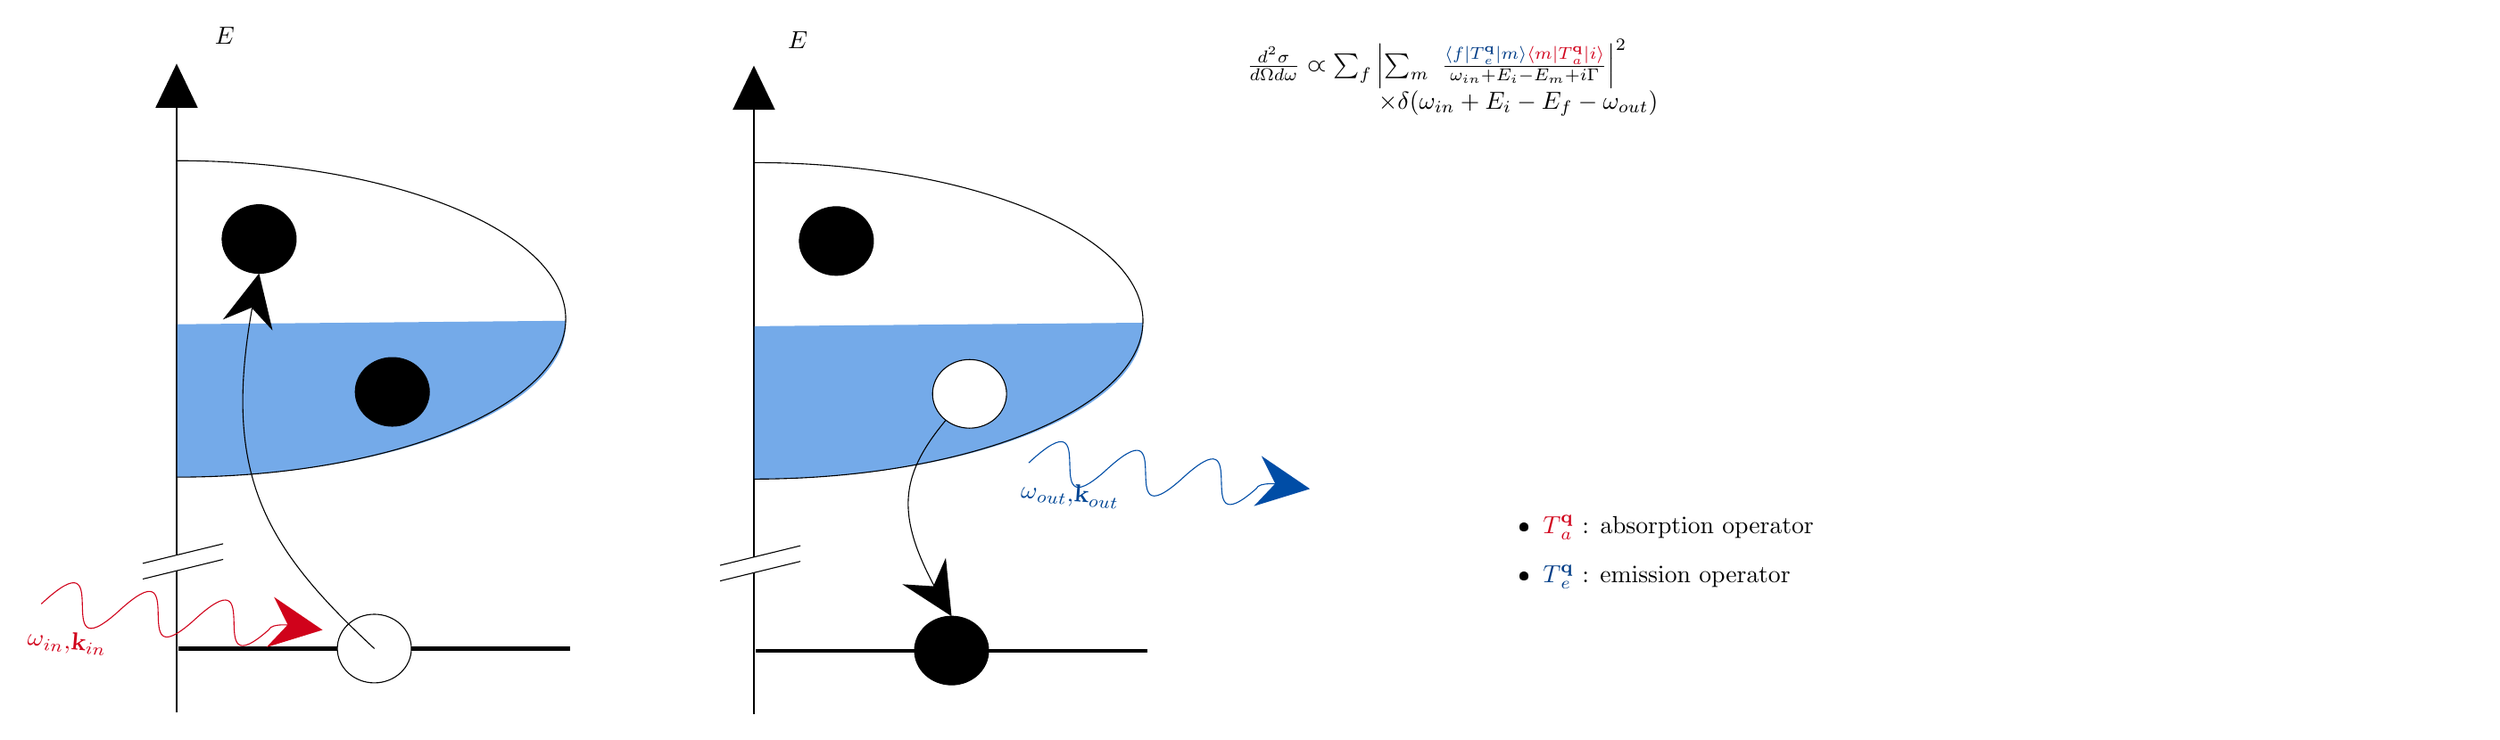
\begin{tikzpicture}[x=2pt,y=2pt,yscale=-1,xscale=1]
%uncomment if require: \path (0,300); %set diagram left start at 0, and has height of 300

%Straight Lines [id:da1682050496037556] 
\draw    (51.78,48.89) -- (51.78,145.56) ;
\draw [shift={(51.78,45.89)}, rotate = 90] [fill={rgb, 255:red, 0; green, 0; blue, 0 }  ][line width=0.08]  [draw opacity=0] (8.93,-4.29) -- (0,0) -- (8.93,4.29) -- cycle    ;
%Straight Lines [id:da6292409204718364] 
\draw [line width=1.5]    (52.21,164.42) -- (84.32,164.42) ;
%Straight Lines [id:da7706541735708927] 
\draw    (44.93,147.15) -- (61.2,143.18) ;
%Straight Lines [id:da13668954784751886] 
\draw    (44.93,150.33) -- (61.2,146.35) ;
%Straight Lines [id:da9107760943630434] 
\draw    (51.78,148.54) -- (51.78,177.33) ;
%Shape: Pie [id:dp45147234652580204] 
\draw  [draw opacity=0][fill={rgb, 255:red, 74; green, 144; blue, 226 }  ,fill opacity=0.77 ] (130.55,97.99) .. controls (130.56,98.23) and (130.57,98.46) .. (130.57,98.7) .. controls (130.57,115.81) and (95.29,129.68) .. (51.78,129.68) -- (51.78,98.7) -- cycle ;
%Shape: Chord [id:dp6727201582698153] 
\draw   (51.78,129.68) .. controls (95.29,129.68) and (130.57,115.32) .. (130.57,97.61) .. controls (130.57,79.9) and (95.29,65.55) .. (51.78,65.55) -- cycle ;
%Shape: Ellipse [id:dp049675451296523954] 
\draw   (84.32,164.42) .. controls (84.32,160.58) and (87.68,157.47) .. (91.82,157.47) .. controls (95.96,157.47) and (99.31,160.58) .. (99.31,164.42) .. controls (99.31,168.26) and (95.96,171.37) .. (91.82,171.37) .. controls (87.68,171.37) and (84.32,168.26) .. (84.32,164.42) -- cycle ;
%Straight Lines [id:da8500849887599712] 
\draw [line width=1.5]    (99.31,164.42) -- (131.42,164.42) ;
%Curve Lines [id:da7647855933040957] 
\draw    (91.82,164.42) .. controls (68.65,142.93) and (60.34,128.05) .. (67.87,91.25) ;
\draw [shift={(68.48,88.38)}, rotate = 102.41] [fill={rgb, 255:red, 0; green, 0; blue, 0 }  ][line width=0.08]  [draw opacity=0] (10.72,-5.15) -- (0,0) -- (10.72,5.15) -- (7.12,0) -- cycle    ;
%Shape: Ellipse [id:dp15457278262908036] 
\draw  [fill={rgb, 255:red, 0; green, 0; blue, 0 }  ,fill opacity=1 ] (60.99,81.43) .. controls (60.99,77.59) and (64.34,74.48) .. (68.48,74.48) .. controls (72.62,74.48) and (75.98,77.59) .. (75.98,81.43) .. controls (75.98,85.27) and (72.62,88.38) .. (68.48,88.38) .. controls (64.34,88.38) and (60.99,85.27) .. (60.99,81.43) -- cycle ;
%Curve Lines [id:da12990763439089414] 
\draw [color={rgb, 255:red, 208; green, 2; blue, 27 }  ,draw opacity=1 ]   (24.38,155.37) .. controls (40.15,140.64) and (25.63,169.6) .. (39.73,157.12) ;
%Curve Lines [id:da36238954486185093] 
\draw [color={rgb, 255:red, 208; green, 2; blue, 27 }  ,draw opacity=1 ]   (39.73,157.12) .. controls (55.5,142.39) and (40.98,171.35) .. (55.08,158.87) ;
%Curve Lines [id:da036229838871078335] 
\draw [color={rgb, 255:red, 208; green, 2; blue, 27 }  ,draw opacity=1 ]   (55.08,158.87) .. controls (70.85,144.14) and (56.33,173.1) .. (70.43,160.62) ;
%Curve Lines [id:da47740550792609604] 
\draw [color={rgb, 255:red, 208; green, 2; blue, 27 }  ,draw opacity=1 ]   (70.43,160.62) .. controls (71.06,159.11) and (75.06,159.61) .. (78.41,160.16) ;
\draw [shift={(81.33,160.65)}, rotate = 188.55] [fill={rgb, 255:red, 208; green, 2; blue, 27 }  ,fill opacity=1 ][line width=0.08]  [draw opacity=0] (10.72,-5.15) -- (0,0) -- (10.72,5.15) -- (7.12,0) -- cycle    ;
%Shape: Ellipse [id:dp42273501149910286] 
\draw  [fill={rgb, 255:red, 0; green, 0; blue, 0 }  ,fill opacity=1 ] (87.96,112.4) .. controls (87.96,108.57) and (91.32,105.45) .. (95.46,105.45) .. controls (99.6,105.45) and (102.95,108.57) .. (102.95,112.4) .. controls (102.95,116.24) and (99.6,119.35) .. (95.46,119.35) .. controls (91.32,119.35) and (87.96,116.24) .. (87.96,112.4) -- cycle ;
%Straight Lines [id:da6697130366412348] 
\draw    (168.67,49.29) -- (168.67,145.96) ;
\draw [shift={(168.67,46.29)}, rotate = 90] [fill={rgb, 255:red, 0; green, 0; blue, 0 }  ][line width=0.08]  [draw opacity=0] (8.93,-4.29) -- (0,0) -- (8.93,4.29) -- cycle    ;
%Straight Lines [id:da3802170758863853] 
\draw [line width=1.5]    (169.1,164.82) -- (201.21,164.82) ;
%Straight Lines [id:da8489792381049942] 
\draw    (161.82,147.55) -- (178.09,143.58) ;
%Straight Lines [id:da46150923563297575] 
\draw    (161.82,150.72) -- (178.09,146.75) ;
%Straight Lines [id:da6387795198494673] 
\draw    (168.67,148.94) -- (168.67,177.73) ;
%Shape: Pie [id:dp30948132213158974] 
\draw  [draw opacity=0][fill={rgb, 255:red, 74; green, 144; blue, 226 }  ,fill opacity=0.77 ] (247.44,98.39) .. controls (247.45,98.62) and (247.46,98.86) .. (247.46,99.1) .. controls (247.46,116.21) and (212.18,130.07) .. (168.67,130.07) -- (168.67,99.1) -- cycle ;
%Shape: Chord [id:dp6739682604362284] 
\draw   (168.67,130.07) .. controls (212.18,130.07) and (247.46,115.72) .. (247.46,98.01) .. controls (247.46,80.3) and (212.18,65.94) .. (168.67,65.94) -- cycle ;
%Shape: Ellipse [id:dp8671135752553624] 
\draw  [fill={rgb, 255:red, 0; green, 0; blue, 0 }  ,fill opacity=1 ] (201.21,164.82) .. controls (201.21,160.98) and (204.57,157.87) .. (208.71,157.87) .. controls (212.85,157.87) and (216.2,160.98) .. (216.2,164.82) .. controls (216.2,168.66) and (212.85,171.77) .. (208.71,171.77) .. controls (204.57,171.77) and (201.21,168.66) .. (201.21,164.82) -- cycle ;
%Straight Lines [id:da8595180597244783] 
\draw [line width=1.5]    (216.2,164.82) -- (248.31,164.82) ;
%Curve Lines [id:da8725928953181541] 
\draw    (212.35,112.8) .. controls (197.96,127.86) and (195.81,135.78) .. (207.21,155.36) ;
\draw [shift={(208.71,157.87)}, rotate = 238.66] [fill={rgb, 255:red, 0; green, 0; blue, 0 }  ][line width=0.08]  [draw opacity=0] (10.72,-5.15) -- (0,0) -- (10.72,5.15) -- (7.12,0) -- cycle    ;
%Shape: Ellipse [id:dp9585262566478759] 
\draw  [fill={rgb, 255:red, 0; green, 0; blue, 0 }  ,fill opacity=1 ] (177.88,81.83) .. controls (177.88,77.99) and (181.23,74.88) .. (185.37,74.88) .. controls (189.51,74.88) and (192.87,77.99) .. (192.87,81.83) .. controls (192.87,85.67) and (189.51,88.78) .. (185.37,88.78) .. controls (181.23,88.78) and (177.88,85.67) .. (177.88,81.83) -- cycle ;
%Curve Lines [id:da3221480472936924] 
\draw [color={rgb, 255:red, 0; green, 77; blue, 166 }  ,draw opacity=1 ]   (224.34,126.78) .. controls (240.1,112.05) and (225.58,141.01) .. (239.69,128.53) ;
%Curve Lines [id:da45318779110131835] 
\draw [color={rgb, 255:red, 0; green, 77; blue, 166 }  ,draw opacity=1 ]   (239.69,128.53) .. controls (255.45,113.8) and (240.93,142.76) .. (255.04,130.28) ;
%Curve Lines [id:da3313125868245088] 
\draw [color={rgb, 255:red, 0; green, 77; blue, 166 }  ,draw opacity=1 ]   (255.04,130.28) .. controls (270.8,115.55) and (256.28,144.51) .. (270.39,132.02) ;
%Curve Lines [id:da5988032124204304] 
\draw [color={rgb, 255:red, 0; green, 77; blue, 166 }  ,draw opacity=1 ]   (270.39,132.02) .. controls (271.02,130.52) and (275.01,131.02) .. (278.36,131.57) ;
\draw [shift={(281.28,132.06)}, rotate = 188.55] [fill={rgb, 255:red, 0; green, 77; blue, 166 }  ,fill opacity=1 ][line width=0.08]  [draw opacity=0] (10.72,-5.15) -- (0,0) -- (10.72,5.15) -- (7.12,0) -- cycle    ;
%Shape: Ellipse [id:dp16915890401253364] 
\draw  [fill={rgb, 255:red, 255; green, 255; blue, 255 }  ,fill opacity=1 ] (204.85,112.8) .. controls (204.85,108.96) and (208.21,105.85) .. (212.35,105.85) .. controls (216.49,105.85) and (219.84,108.96) .. (219.84,112.8) .. controls (219.84,116.64) and (216.49,119.75) .. (212.35,119.75) .. controls (208.21,119.75) and (204.85,116.64) .. (204.85,112.8) -- cycle ;

% Text Node
\draw (21.39,159.77) node [anchor=north west][inner sep=0.75pt]  [rotate=-5.19]  {$\textcolor[rgb]{0.82,0.01,0.11}{\omega }\textcolor[rgb]{0.82,0.01,0.11}{_{in}}\textcolor[rgb]{0.82,0.01,0.11}{,}\mathbf{\textcolor[rgb]{0.82,0.01,0.11}{k}}\textcolor[rgb]{0.82,0.01,0.11}{_{in}}$};
% Text Node
\draw (222.51,129.84) node [anchor=north west][inner sep=0.75pt]  [rotate=-4.49]  {$\textcolor[rgb]{0,0.27,0.58}{\omega }\textcolor[rgb]{0,0.27,0.58}{_{out}}\textcolor[rgb]{0,0.27,0.58}{,}\mathbf{\textcolor[rgb]{0,0.27,0.58}{k}}\textcolor[rgb]{0,0.27,0.58}{_{out}}$};
% Text Node
\draw (59.06,38.09) node [anchor=north west][inner sep=0.75pt]    {$E$};
% Text Node
\draw (175.09,38.89) node [anchor=north west][inner sep=0.75pt]    {$E$};
% Text Node
\draw (265.5,40.4) node [anchor=north west][inner sep=0.75pt]    {$ \begin{array}{l}
\frac{d^{2} \sigma }{d\Omega d\omega } \varpropto \sum _{f}\left| \sum _{m} \ \frac{\textcolor[rgb]{0,0.24,0.53}{\langle f|T}\textcolor[rgb]{0,0.24,0.53}{_{e}^{\mathbf{q}}}\textcolor[rgb]{0,0.24,0.53}{|m\rangle }\textcolor[rgb]{0.82,0.01,0.11}{\langle m|T}\textcolor[rgb]{0.82,0.01,0.11}{_{a}^{\mathbf{q}}}\textcolor[rgb]{0.82,0.01,0.11}{|i\rangle }}{\omega _{in} +E_{i} -E_{m} +i\Gamma }\right| ^{2}\\
\ \ \ \ \ \ \ \ \ \ \ \ \ \ \ \ \times \delta ( \omega _{in} +E_{i} -E_{f} -\omega _{out})
\end{array}$};
% Text Node
\draw (315.5,137) node[
    anchor=north west,
    inner sep=0.75pt,
    align=left
] {
    \begin{minipage}{14cm}
        \begin{itemize}
            \item $\displaystyle \textcolor[rgb]{0.82,0.01,0.11}{T}\textcolor[rgb]{0.82,0.01,0.11}{_{a}^{\mathbf{q}}}$ : absorption operator
            \item $\displaystyle \textcolor[rgb]{0,0.24,0.53}{T}\textcolor[rgb]{0,0.24,0.53}{_{e}^{\mathbf{q}}}$ : emission operator
        \end{itemize}
    \end{minipage}
};


\end{tikzpicture}


\end{minipage}

\vspace{0.5em}

\begin{minipage}{0.39\textwidth}
\begin{itemize}
\item $E_i, |i\rangle$ : ground state
\item $\Gamma$ : quasiparticle lifetime
\end{itemize}
\end{minipage}
\begin{minipage}{0.53\textwidth}
\begin{itemize}
\item $E_m, |m\rangle$ : intermediate state (left Fig.)
\item $E_f, |f\rangle$ : final state (right Fig.)
\end{itemize}
\end{minipage}
\end{beamercolorbox}
\end{block}
\end{column}

\begin{column}{.02\textwidth}
\end{column}	%Empty spacer column in the middle
\begin{column}{.47\textwidth}
\begin{block}{\color{ta2orange!0} Augmented Anderson Impurity Model (AAIM)}
\setbeamercolor{coloredboxstuff}{bg=ta2orange!0}
\begin{beamercolorbox}[wd=\textwidth]{coloredboxstuff}
The model of interest is the AAIM, corresponding to an impurity with \textcolor[rgb]{0.25,0.46,0.02}{\textbf{core}} and \textcolor[rgb]{0,0.32,0.69}{\textbf{valence}} states, the latter hybridizing with a \textcolor[rgb]{0.75,0.47,0}{\textbf{non-interacting bath}}.

\vspace{0.1em}

\begin{minipage}[c]{0.96\textwidth}
\centering


\tikzset{every picture/.style={line width=0.75pt}} %set default line width to 0.75pt        

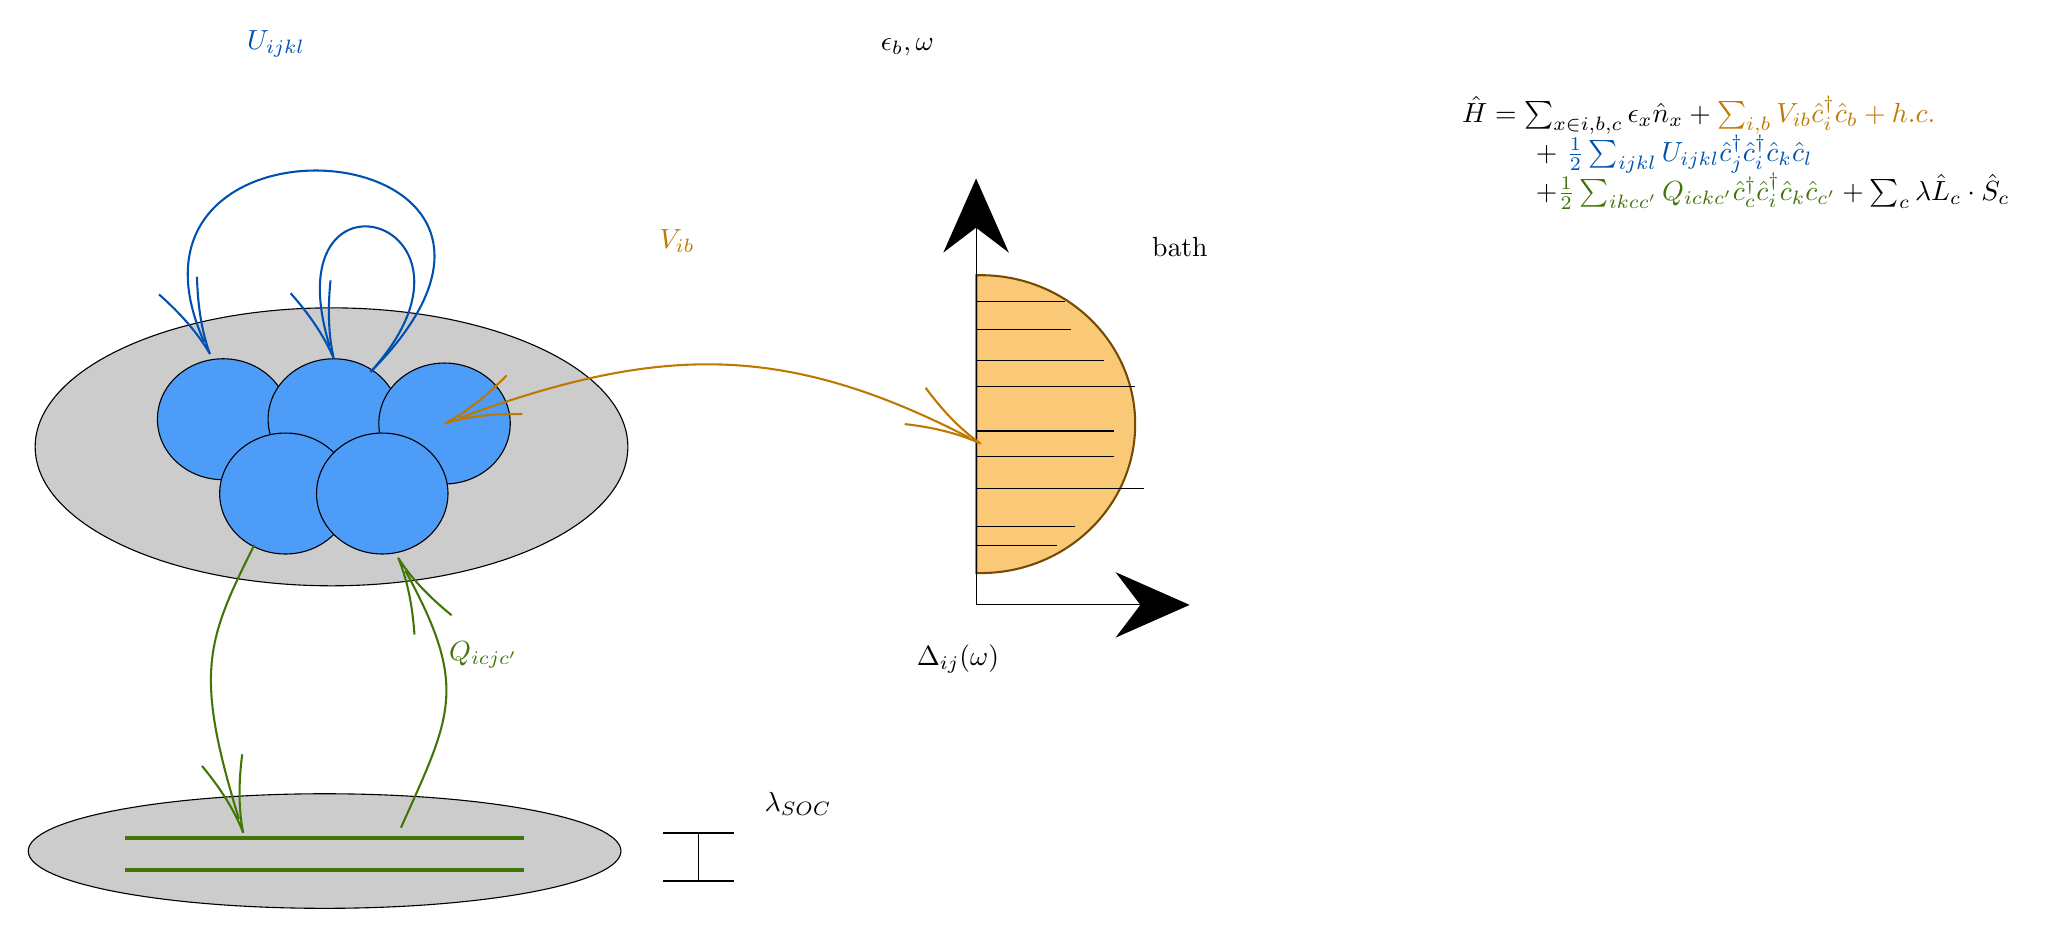
\begin{tikzpicture}[x=2.5pt,y=2.3pt,yscale=-1,xscale=1]
%uncomment if require: \path (0,330); %set diagram left start at 0, and has height of 330

%Shape: Chord [id:dp25440956650596025] 
\draw  [color={rgb, 255:red, 116; green, 75; blue, 0 }  ,draw opacity=1 ][fill={rgb, 255:red, 245; green, 166; blue, 35 }  ,fill opacity=0.61 ][line width=0.75]  (261.38,130.99) .. controls (261.59,131) and (261.79,131) .. (262,131) .. controls (274.33,131) and (284.33,120.52) .. (284.33,107.6) .. controls (284.33,94.68) and (274.33,84.2) .. (262,84.2) .. controls (261.79,84.2) and (261.57,84.2) .. (261.36,84.21) -- cycle ;
%Shape: Ellipse [id:dp37682332865497914] 
\draw  [fill={rgb, 255:red, 155; green, 155; blue, 155 }  ,fill opacity=0.51 ] (125.33,111.17) .. controls (125.33,99.11) and (144.51,89.33) .. (168.17,89.33) .. controls (191.82,89.33) and (211,99.11) .. (211,111.17) .. controls (211,123.22) and (191.82,133) .. (168.17,133) .. controls (144.51,133) and (125.33,123.22) .. (125.33,111.17) -- cycle ;
%Shape: Circle [id:dp5397571863840275] 
\draw  [fill={rgb, 255:red, 77; green, 156; blue, 247 }  ,fill opacity=1 ] (143,106.83) .. controls (143,101.59) and (147.25,97.33) .. (152.5,97.33) .. controls (157.75,97.33) and (162,101.59) .. (162,106.83) .. controls (162,112.08) and (157.75,116.33) .. (152.5,116.33) .. controls (147.25,116.33) and (143,112.08) .. (143,106.83) -- cycle ;
%Shape: Circle [id:dp17885792014597746] 
\draw  [fill={rgb, 255:red, 77; green, 156; blue, 247 }  ,fill opacity=1 ] (159,106.83) .. controls (159,101.59) and (163.25,97.33) .. (168.5,97.33) .. controls (173.75,97.33) and (178,101.59) .. (178,106.83) .. controls (178,112.08) and (173.75,116.33) .. (168.5,116.33) .. controls (163.25,116.33) and (159,112.08) .. (159,106.83) -- cycle ;
%Shape: Circle [id:dp640001436758383] 
\draw  [fill={rgb, 255:red, 77; green, 156; blue, 247 }  ,fill opacity=1 ] (175,107.5) .. controls (175,102.25) and (179.25,98) .. (184.5,98) .. controls (189.75,98) and (194,102.25) .. (194,107.5) .. controls (194,112.75) and (189.75,117) .. (184.5,117) .. controls (179.25,117) and (175,112.75) .. (175,107.5) -- cycle ;
%Shape: Circle [id:dp18860372246468882] 
\draw  [fill={rgb, 255:red, 77; green, 156; blue, 247 }  ,fill opacity=1 ] (152,118.5) .. controls (152,113.25) and (156.25,109) .. (161.5,109) .. controls (166.75,109) and (171,113.25) .. (171,118.5) .. controls (171,123.75) and (166.75,128) .. (161.5,128) .. controls (156.25,128) and (152,123.75) .. (152,118.5) -- cycle ;
%Shape: Circle [id:dp921087155303204] 
\draw  [fill={rgb, 255:red, 77; green, 156; blue, 247 }  ,fill opacity=1 ] (166,118.5) .. controls (166,113.25) and (170.25,109) .. (175.5,109) .. controls (180.75,109) and (185,113.25) .. (185,118.5) .. controls (185,123.75) and (180.75,128) .. (175.5,128) .. controls (170.25,128) and (166,123.75) .. (166,118.5) -- cycle ;
%Shape: Ellipse [id:dp7663776704708546] 
\draw  [fill={rgb, 255:red, 155; green, 155; blue, 155 }  ,fill opacity=0.51 ] (124.33,174.67) .. controls (124.33,169.7) and (143.51,165.67) .. (167.17,165.67) .. controls (190.82,165.67) and (210,169.7) .. (210,174.67) .. controls (210,179.64) and (190.82,183.67) .. (167.17,183.67) .. controls (143.51,183.67) and (124.33,179.64) .. (124.33,174.67) -- cycle ;
%Straight Lines [id:da5175903267304353] 
\draw [color={rgb, 255:red, 65; green, 117; blue, 5 }  ,draw opacity=1 ][line width=1.5]    (138.33,172.67) -- (196,172.67) ;
%Straight Lines [id:da284089715682998] 
\draw [color={rgb, 255:red, 65; green, 117; blue, 5 }  ,draw opacity=1 ][line width=1.5]    (138.33,177.67) -- (196,177.67) ;
%Straight Lines [id:da7488434292275031] 
\draw    (261.33,72) -- (261.33,136) ;
\draw [shift={(261.33,69)}, rotate = 90] [fill={rgb, 255:red, 0; green, 0; blue, 0 }  ][line width=0.08]  [draw opacity=0] (10.72,-5.15) -- (0,0) -- (10.72,5.15) -- (7.12,0) -- cycle    ;
%Straight Lines [id:da6532929815979057] 
\draw    (289.2,136) -- (280,136) -- (261.33,136) ;
\draw [shift={(292.2,136)}, rotate = 180] [fill={rgb, 255:red, 0; green, 0; blue, 0 }  ][line width=0.08]  [draw opacity=0] (10.72,-5.15) -- (0,0) -- (10.72,5.15) -- (7.12,0) -- cycle    ;
%Straight Lines [id:da7050392783676652] 
\draw    (261.33,126.67) -- (273,126.67) ;
%Straight Lines [id:da3983025861719506] 
\draw    (261.33,123.67) -- (275.67,123.67) ;
%Straight Lines [id:da7534826824723967] 
\draw    (261.33,117.67) -- (285.67,117.67) ;
%Straight Lines [id:da5752820133880527] 
\draw    (261.33,112.67) -- (281.33,112.67) ;
%Straight Lines [id:da09984115289873852] 
\draw    (261.33,108.67) -- (281.33,108.67) ;
%Straight Lines [id:da05955355663491346] 
\draw    (261.33,101.67) -- (284.33,101.67) ;
%Straight Lines [id:da9761346478021231] 
\draw    (261.33,97.67) -- (279.8,97.67) ;
%Straight Lines [id:da19834353022102214] 
\draw    (261.33,92.67) -- (275,92.67) ;
%Curve Lines [id:da4838231435704238] 
\draw [color={rgb, 255:red, 190; green, 120; blue, 0 }  ,draw opacity=1 ][line width=0.75]    (186.77,106.58) .. controls (215.34,95.2) and (233.38,94.63) .. (260.34,109.72) ;
\draw [shift={(262,110.67)}, rotate = 209.93] [color={rgb, 255:red, 190; green, 120; blue, 0 }  ,draw opacity=1 ][line width=0.75]    (10.93,-3.29) .. controls (6.95,-1.4) and (3.31,-0.3) .. (0,0) .. controls (3.31,0.3) and (6.95,1.4) .. (10.93,3.29)   ;
\draw [shift={(184.5,107.5)}, rotate = 337.71] [color={rgb, 255:red, 190; green, 120; blue, 0 }  ,draw opacity=1 ][line width=0.75]    (10.93,-3.29) .. controls (6.95,-1.4) and (3.31,-0.3) .. (0,0) .. controls (3.31,0.3) and (6.95,1.4) .. (10.93,3.29)   ;
%Curve Lines [id:da1595481029803827] 
\draw [color={rgb, 255:red, 0; green, 81; blue, 175 }  ,draw opacity=1 ][line width=0.75]    (167.91,95.4) .. controls (159.23,64.64) and (193.79,75.49) .. (173.8,99.4) ;
\draw [shift={(168.5,97.33)}, rotate = 252.1] [color={rgb, 255:red, 0; green, 81; blue, 175 }  ,draw opacity=1 ][line width=0.75]    (10.93,-3.29) .. controls (6.95,-1.4) and (3.31,-0.3) .. (0,0) .. controls (3.31,0.3) and (6.95,1.4) .. (10.93,3.29)   ;
%Curve Lines [id:da5704274989974883] 
\draw [color={rgb, 255:red, 0; green, 81; blue, 175 }  ,draw opacity=1 ][line width=0.75]    (149.78,94.74) .. controls (133.31,54.8) and (208.47,61.58) .. (173.8,99.4) ;
\draw [shift={(150.6,96.6)}, rotate = 244.98] [color={rgb, 255:red, 0; green, 81; blue, 175 }  ,draw opacity=1 ][line width=0.75]    (10.93,-3.29) .. controls (6.95,-1.4) and (3.31,-0.3) .. (0,0) .. controls (3.31,0.3) and (6.95,1.4) .. (10.93,3.29)   ;
%Curve Lines [id:da1345648493310485] 
\draw [color={rgb, 255:red, 65; green, 117; blue, 5 }  ,draw opacity=1 ][line width=0.75]    (154.78,169.62) .. controls (148.3,146.7) and (150.02,141.73) .. (157,126.6) ;
\draw [shift={(155.4,171.8)}, rotate = 253.81] [color={rgb, 255:red, 65; green, 117; blue, 5 }  ,draw opacity=1 ][line width=0.75]    (10.93,-3.29) .. controls (6.95,-1.4) and (3.31,-0.3) .. (0,0) .. controls (3.31,0.3) and (6.95,1.4) .. (10.93,3.29)   ;
%Curve Lines [id:da6604273168760524] 
\draw [color={rgb, 255:red, 65; green, 117; blue, 5 }  ,draw opacity=1 ][line width=0.75]    (178.85,130.64) .. controls (188.03,148.9) and (185.53,153.24) .. (178.2,171) ;
\draw [shift={(177.8,128.6)}, rotate = 62.53] [color={rgb, 255:red, 65; green, 117; blue, 5 }  ,draw opacity=1 ][line width=0.75]    (10.93,-3.29) .. controls (6.95,-1.4) and (3.31,-0.3) .. (0,0) .. controls (3.31,0.3) and (6.95,1.4) .. (10.93,3.29)   ;
%Straight Lines [id:da012051238858155178] 
\draw    (261.33,88.27) -- (274.2,88.27) ;
%Straight Lines [id:da6235189352581033] 
\draw    (221.2,171.8) -- (221.2,179.4) ;
\draw [shift={(221.2,179.4)}, rotate = 270] [color={rgb, 255:red, 0; green, 0; blue, 0 }  ][line width=0.75]    (0,5.59) -- (0,-5.59)   ;
\draw [shift={(221.2,171.8)}, rotate = 270] [color={rgb, 255:red, 0; green, 0; blue, 0 }  ][line width=0.75]    (0,5.59) -- (0,-5.59)   ;

% Text Node
\draw (215.2,76.6) node [anchor=north west][inner sep=0.75pt]    {$\textcolor[rgb]{0.75,0.47,0}{V_{ib}}$};
% Text Node
\draw (155.6,45.4) node [anchor=north west][inner sep=0.75pt]    {$\textcolor[rgb]{0,0.32,0.69}{U_{ijkl}}$};
% Text Node
\draw (184.8,141.4) node [anchor=north west][inner sep=0.75pt]    {$\textcolor[rgb]{0.25,0.46,0.02}{Q_{icjc'}}$};
% Text Node
\draw (230.4,165) node [anchor=north west][inner sep=0.75pt]    {$\lambda _{SOC}$};
% Text Node
\draw (252.4,141.8) node [anchor=north west][inner sep=0.75pt]    {$\Delta _{ij}( \omega )$};
% Text Node
\draw (247.2,46.6) node [anchor=north west][inner sep=0.75pt]    {$\epsilon _{b} ,\omega $};
% Text Node
\draw (292.3,79.7) node   [align=left] {\begin{minipage}[lt]{27.61pt}\setlength\topsep{0pt}
bath
\end{minipage}};
% Text Node
\draw (329.2,55.6) node [anchor=north west][inner sep=0.75pt]    {$ \begin{array}{l}
\hat{H} =\sum _{x\in i,b,c} \epsilon _{x}\hat{n}_{x} +\textcolor[rgb]{0.75,0.47,0}{\sum _{i,b} V_{ib}\hat{c}_{i}^{\dagger }\hat{c}_{b} +h.c.}\\
\ \ \ \ \ \ \ \ +\ \textcolor[rgb]{0,0.32,0.69}{\frac{1}{2}\sum _{ijkl} U_{ijkl}\hat{c}_{j}^{\dagger }\hat{c}_{i}^{\dagger }\hat{c}_{k}\hat{c}_{l}}\\
\ \ \ \ \ \ \ \ +\textcolor[rgb]{0.25,0.46,0.02}{\frac{1}{2}\sum _{ikcc'} Q_{ickc'}\hat{c}_{c}^{\dagger }\hat{c}_{i}^{\dagger }\hat{c}_{k}\hat{c}_{c'}} +\sum _{c} \lambda \hat{L}_{c} \cdot \hat{S}_{c}
\end{array}$};


\end{tikzpicture}

\end{minipage}

\vspace{0.7em}

\begin{minipage}{0.45 \textwidth}
\textbf{Building the model}
\begin{itemize}
\item Density Functional Theory
\item Dynamical Mean Field Theory
\end{itemize}
\end{minipage}
\begin{minipage}{0.45 \textwidth}
\textbf{Solving the model}
\begin{itemize}
\item Matrix Product State formalism
\item Exact Diagonalization (Lanczos)
\end{itemize}
\end{minipage}

\end{beamercolorbox}
\end{block}
\end{column}

\begin{column}{.03\textwidth}
\end{column} % Empty spacer column

\end{columns} % End of all the columns
\vspace{-0.75em}


%%%%%%%%%%%%%%%%%%%%%%%%%%%%%%%%%%%%%%%%%%%%%%%%%%%%%%%%%%%%%%%%%%
% DFT & DMFT
%%%%%%%%%%%%%%%%%%%%%%%%%%%%%%%%%%%%%%%%%%%%%%%%%%%%%%%


\begin{columns}[t] % The whole poster consists of two major columns, each of which can be subdivided further with another \begin{columns} block - the [t] argument aligns each column's content to the top

\begin{column}{.03\textwidth}
\end{column} % Empty spacer column

\begin{column}{.34\textwidth} % The first column
\begin{block}{\color{cyan!40} Density Functional Theory (DFT)}
\setbeamercolor{coloredboxstuff}{bg=cyan!5}
\begin{beamercolorbox}[wd=\textwidth]{coloredboxstuff}
One band model benchmark with copper oxide CuO.

\vspace{0.15em}

\begin{minipage}{0.96\textwidth}
	\centering
	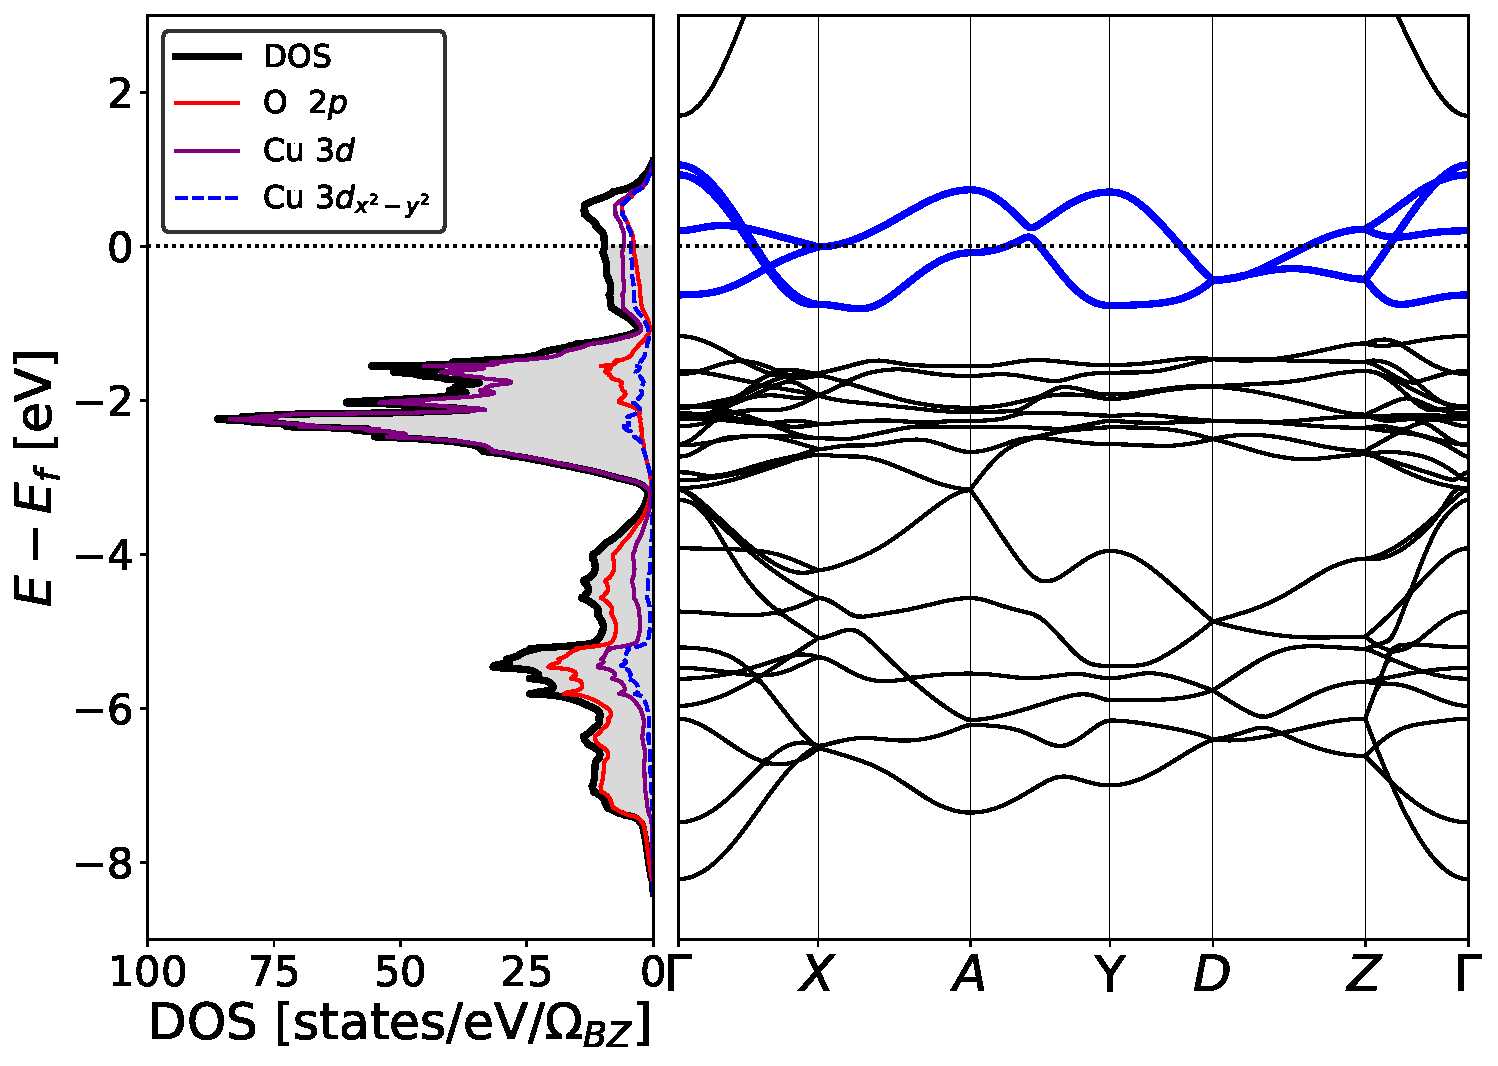
\includegraphics[width=0.95\textwidth]{imgs/dos_vs_bands_PM.pdf}
\end{minipage}

\vspace{0.15em}

\begin{itemize}
	\item \textbf{Metallic phase} altought experiments measure a gap.
	\item Copper $d_{x^2-y^2}$'s hybridize with oxygen $2p$'s at $E_f$.
\end{itemize}
   
\end{beamercolorbox}
\end{block}
\end{column} % End of the middle column
\begin{column}{.017\textwidth}
\end{column}	%Empty spacer column in the middle

\begin{column}{.60\textwidth}
	\begin{block}{\color{cyan!40} Dynamical Mean Field THeory (DMFT)}
	\setbeamercolor{coloredboxstuff}{bg=cyan!5}
	\begin{beamercolorbox}[wd=\textwidth]{coloredboxstuff}
DMFT maps the lattice problem self-consistently onto an impurity model, solved with Monte-Carlo.

\vspace{0.15em}

\hspace{0.02\textwidth}
\begin{minipage}{0.48\textwidth}
	\centering
    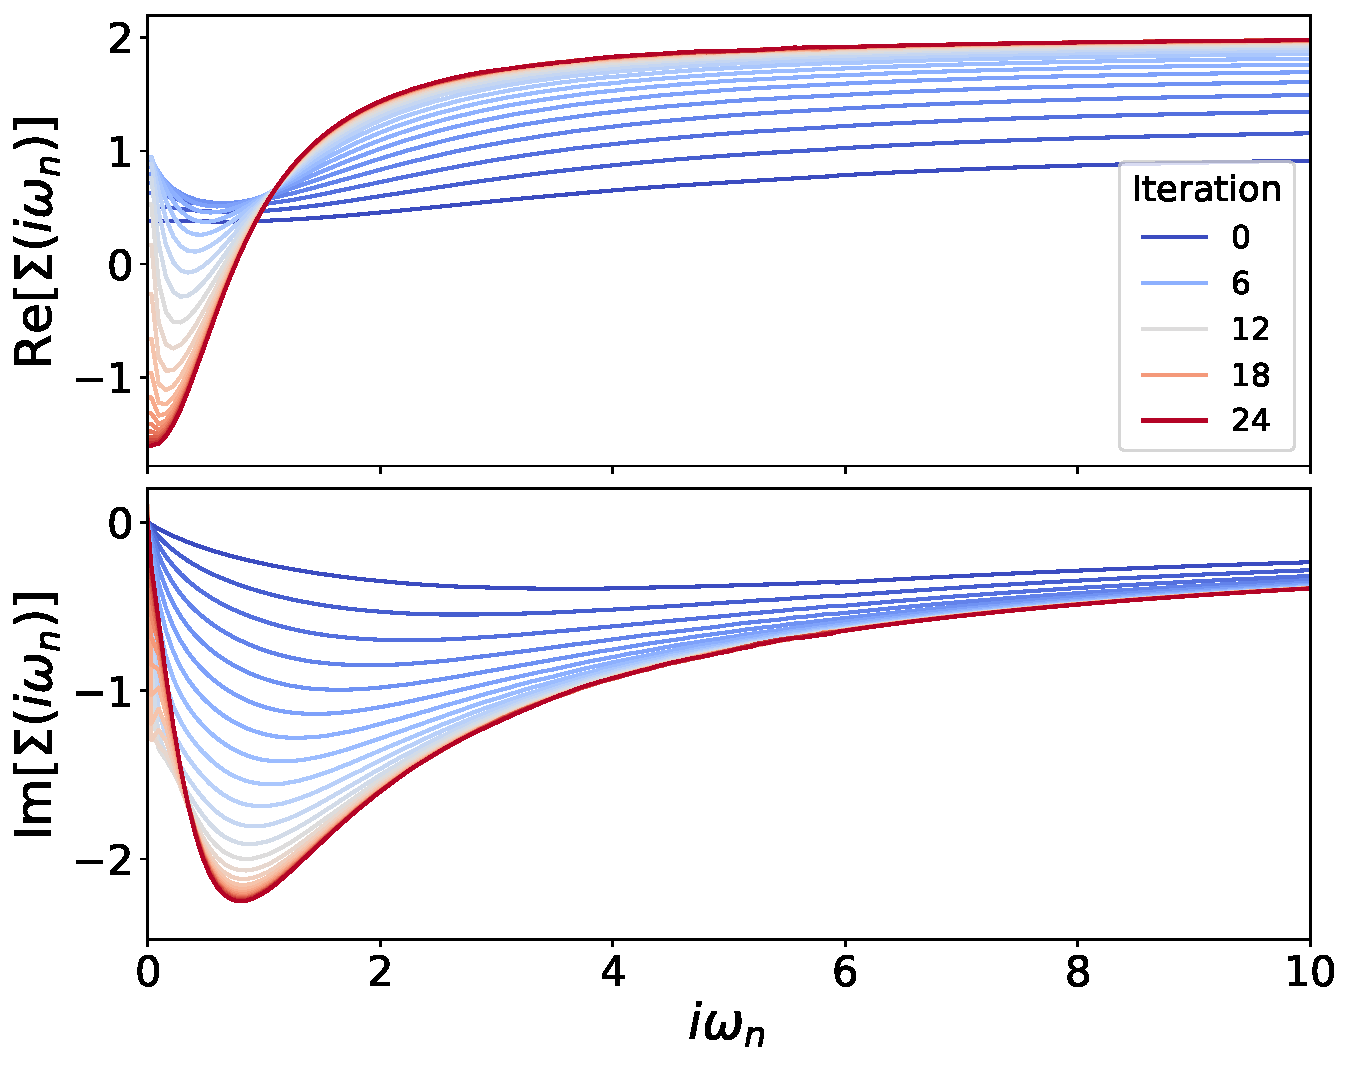
\includegraphics[width=0.95\textwidth]{imgs/SE_iwn.pdf}
\end{minipage}
\hspace{-0.05\textwidth}
\begin{minipage}{0.48\textwidth}
	\centering
	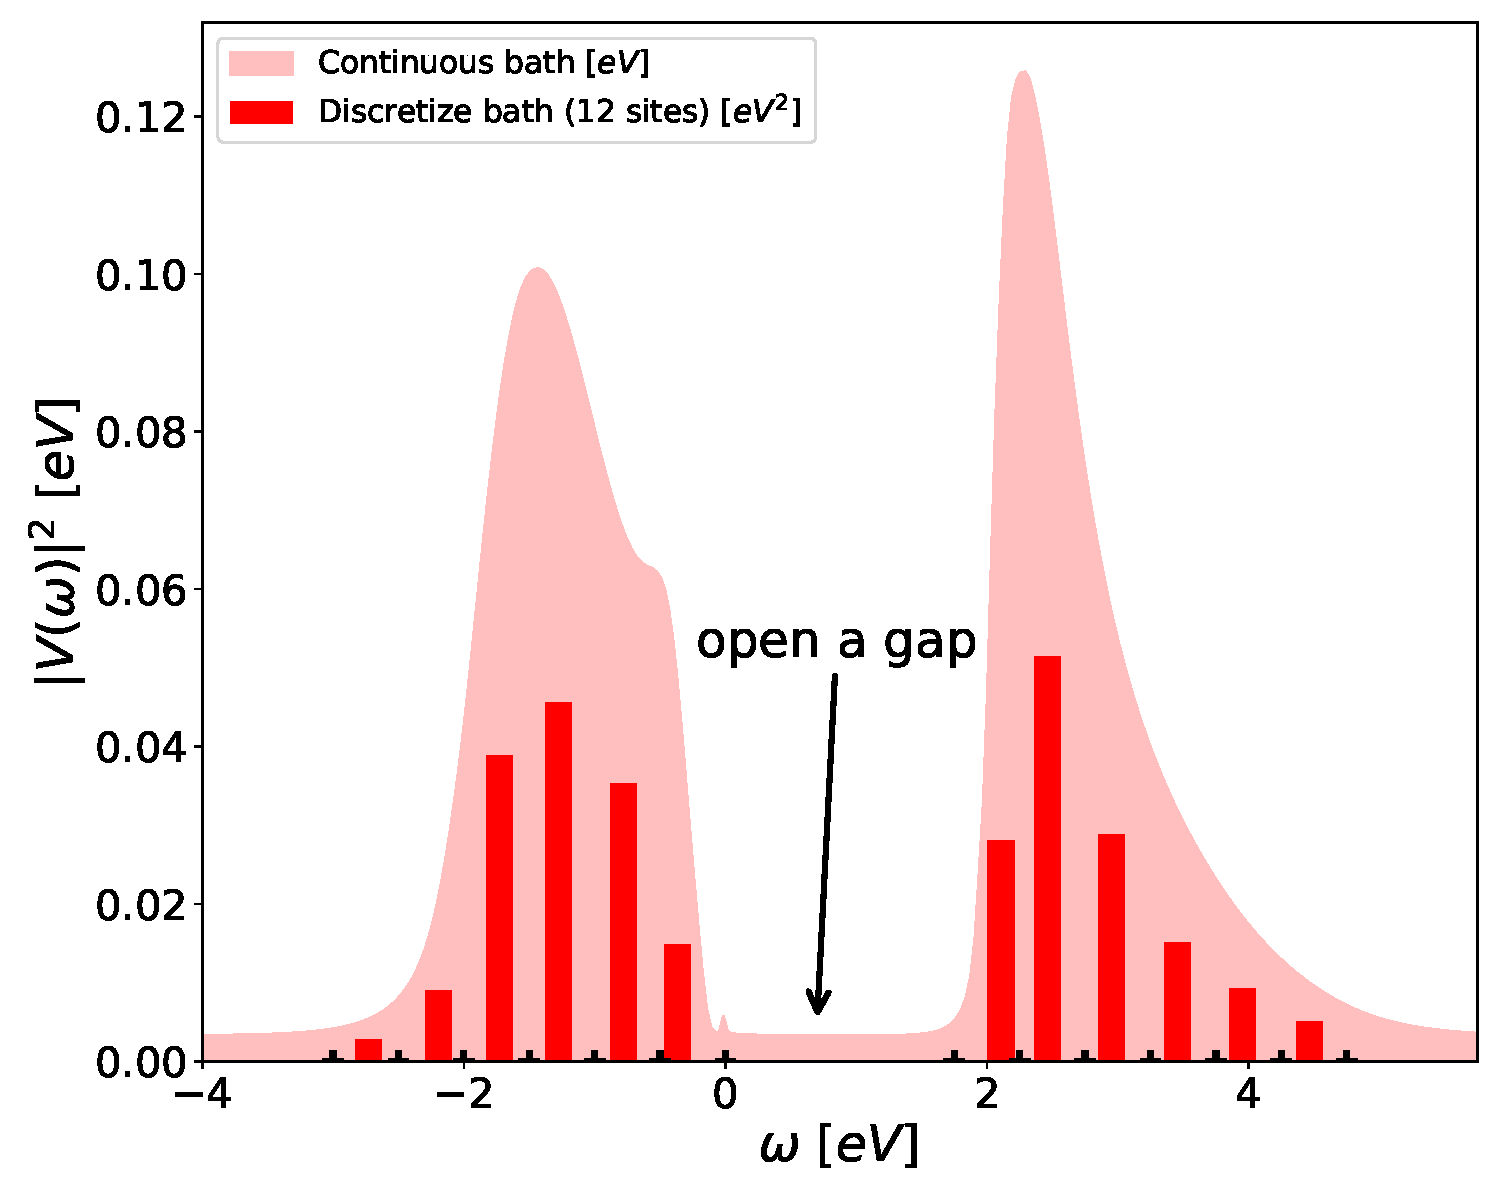
\includegraphics[width=0.92\textwidth]{imgs/discr_bath_N12.pdf}
\end{minipage}

\vspace{0.15em}

\begin{itemize}
\item Extract the converged self-energy $\Sigma(i\omega_n)$ and \textbf{continuate it analytically} to real frequencies.
\item Compute the continuous bath $|V(\omega)|^2 \propto \Im(\Delta(\omega))=G^{-1}(\omega)+\Sigma(\omega)$ and \textbf{discretize it}.
\end{itemize}


	\end{beamercolorbox}
	\end{block}
\end{column}

\begin{column}{.03\textwidth}
\end{column} % Empty spacer column
\end{columns} % End of all the columns in the poster
\vspace{-0.75em}


%%%%%%%%%%%%%%%%%%%%%%%%%%%%%%%%%%%%%%%%%%%%%%%%%%%%%%%%%%%%%%%%%%
% MPS & LANCZOS
%%%%%%%%%%%%%%%%%%%%%%%%%%%%%%%%%%%%%%%%%%%%%%%%%%%%%%%


\begin{columns}[t] % The whole poster consists of two major columns, each of which can be subdivided further with another \begin{columns} block - the [t] argument aligns each column's content to the top

\begin{column}{.03\textwidth}
\end{column} % Empty spacer column

\begin{column}{.33\textwidth} % The first column
\begin{block}{\color{ta2orange!0} Matrix Product States (MPS)}
\setbeamercolor{coloredboxstuff}{bg=ta2orange!0}
\begin{beamercolorbox}[wd=\textwidth]{coloredboxstuff}
A many-body state $| \psi \rangle$ on a basis $|\mathbf{n}=n_1\ldots n_L\rangle$:
\begin{equation*}
|\psi \rangle = \sum_\mathbf{n}c_\mathbf{n} |\mathbf{n}\rangle = \sum_\mathbf{n} \!\!\sum_{a_1\ldots a_{L-1}} \!\! M^{n_1}_{1,a_1}M^{n_2}_{a_1,a_2}\ldots M^{n_L}_{a_{L-1},1} |\mathbf{n}\rangle
\end{equation*}


\begin{minipage}{0.96\textwidth}

\centering

\tikzset{every picture/.style={line width=0.75pt}} %set default line width to 0.75pt        

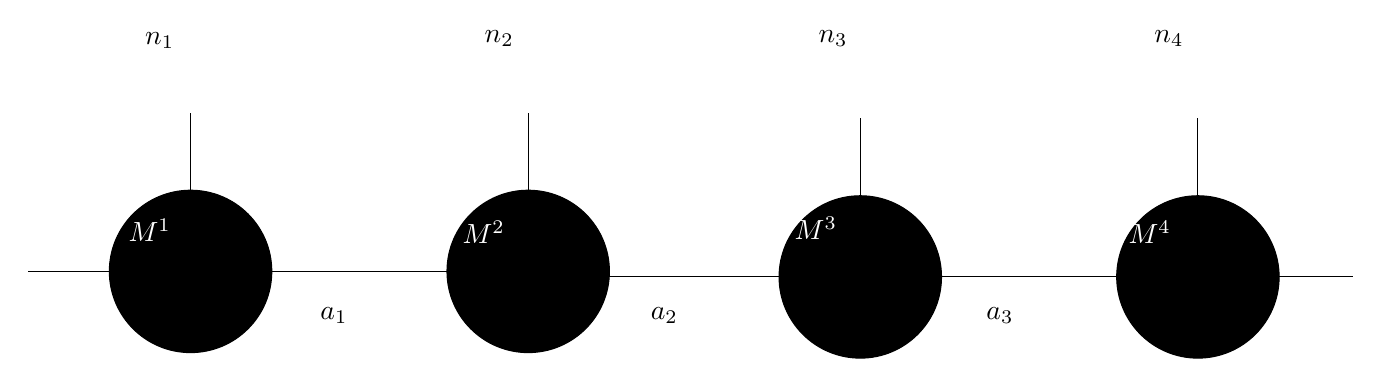
\begin{tikzpicture}[x=2pt,y=2pt,yscale=-1,xscale=1]
%uncomment if require: \path (0,300); %set diagram left start at 0, and has height of 300

%Shape: Circle [id:dp49379703017958154] 
\draw  [fill={rgb, 255:red, 0; green, 0; blue, 0 }  ,fill opacity=1 ] (130.33,130.33) .. controls (130.33,122.23) and (136.9,115.67) .. (145,115.67) .. controls (153.1,115.67) and (159.67,122.23) .. (159.67,130.33) .. controls (159.67,138.43) and (153.1,145) .. (145,145) .. controls (136.9,145) and (130.33,138.43) .. (130.33,130.33) -- cycle ;
%Shape: Circle [id:dp9873366652044924] 
\draw  [fill={rgb, 255:red, 0; green, 0; blue, 0 }  ,fill opacity=1 ] (191.33,130.33) .. controls (191.33,122.23) and (197.9,115.67) .. (206,115.67) .. controls (214.1,115.67) and (220.67,122.23) .. (220.67,130.33) .. controls (220.67,138.43) and (214.1,145) .. (206,145) .. controls (197.9,145) and (191.33,138.43) .. (191.33,130.33) -- cycle ;
%Shape: Circle [id:dp07435353778901121] 
\draw  [fill={rgb, 255:red, 0; green, 0; blue, 0 }  ,fill opacity=1 ] (251.33,131.33) .. controls (251.33,123.23) and (257.9,116.67) .. (266,116.67) .. controls (274.1,116.67) and (280.67,123.23) .. (280.67,131.33) .. controls (280.67,139.43) and (274.1,146) .. (266,146) .. controls (257.9,146) and (251.33,139.43) .. (251.33,131.33) -- cycle ;
%Shape: Circle [id:dp9202175168993141] 
\draw  [fill={rgb, 255:red, 0; green, 0; blue, 0 }  ,fill opacity=1 ] (312.33,131.33) .. controls (312.33,123.23) and (318.9,116.67) .. (327,116.67) .. controls (335.1,116.67) and (341.67,123.23) .. (341.67,131.33) .. controls (341.67,139.43) and (335.1,146) .. (327,146) .. controls (318.9,146) and (312.33,139.43) .. (312.33,131.33) -- cycle ;
%Straight Lines [id:da17544117308797003] 
\draw    (159.67,130.33) -- (191.33,130.33) ;
%Straight Lines [id:da07579848649183252] 
\draw    (219.67,131.33) -- (251.33,131.33) ;
%Straight Lines [id:da7874903524216095] 
\draw    (280.67,131.33) -- (312.33,131.33) ;
%Straight Lines [id:da25077476691990674] 
\draw    (115.67,130.33) -- (130.33,130.33) ;
%Straight Lines [id:da16899996766266256] 
\draw    (341.67,131.33) -- (355,131.33) ;
%Straight Lines [id:da6652772583485322] 
\draw    (145,115.67) -- (145,101.67) ;
%Straight Lines [id:da1663153379537442] 
\draw    (206,115.67) -- (206,101.67) ;
%Straight Lines [id:da82257179464055] 
\draw    (266,116.67) -- (266,102.67) ;
%Straight Lines [id:da9267417672421946] 
\draw    (327,116.67) -- (327,102.67) ;

% Text Node
\draw (133.33,120.4) node [anchor=north west][inner sep=0.75pt]    {$\textcolor[rgb]{1,1,1}{M^{1}}$};
% Text Node
\draw (193.67,120.73) node [anchor=north west][inner sep=0.75pt]    {$\textcolor[rgb]{1,1,1}{M}\textcolor[rgb]{1,1,1}{^{2}}$};
% Text Node
\draw (253.67,120.07) node [anchor=north west][inner sep=0.75pt]    {$\textcolor[rgb]{1,1,1}{M}\textcolor[rgb]{1,1,1}{^{3}}$};
% Text Node
\draw (314,120.73) node [anchor=north west][inner sep=0.75pt]    {$\textcolor[rgb]{1,1,1}{M}\textcolor[rgb]{1,1,1}{^{4}}$};
% Text Node
\draw (168,136.4) node [anchor=north west][inner sep=0.75pt]    {$a_{1}$};
% Text Node
\draw (227.67,136.4) node [anchor=north west][inner sep=0.75pt]    {$a_{2}$};
% Text Node
\draw (288.33,136.4) node [anchor=north west][inner sep=0.75pt]    {$a_{3}$};
% Text Node
\draw (136.33,86.73) node [anchor=north west][inner sep=0.75pt]    {$n_{1}$};
% Text Node
\draw (197.67,86.4) node [anchor=north west][inner sep=0.75pt]    {$n_{2}$};
% Text Node
\draw (258,86.4) node [anchor=north west][inner sep=0.75pt]    {$n_{3}$};
% Text Node
\draw (318.67,86.4) node [anchor=north west][inner sep=0.75pt]    {$n_{4}$};


\end{tikzpicture}

\end{minipage}

\vspace{0.8em}

\begin{itemize}
	\item MPS $=$ chain of rank-3 tensors $M^i$ with dimension that grows exponentially with $L$.
	\item \textbf{Truncating the singular values:} $L{\chi}^2$ complexity while keeping (hopefully) the interesting physics!
	\item $\chi$, that is the number of singular values kept, controll this compression.
\end{itemize}
\end{beamercolorbox}
\end{block}
\end{column} % End of the middle column

\begin{column}{.017\textwidth}
\end{column}	%Empty spacer column in the middle

\begin{column}{.38\textwidth}
	\begin{block}{\color{cyan!40}Density Matrix Renormalization Group}
	\setbeamercolor{coloredboxstuff}{bg=cyan!5}
	\begin{beamercolorbox}[wd=\textwidth]{coloredboxstuff}
Density Matrix Renormalisation Group (DMRG) is a variational method using MPS that allows to compute the ground state.

\vspace{0.5em}

\begin{minipage}{0.60\textwidth}
	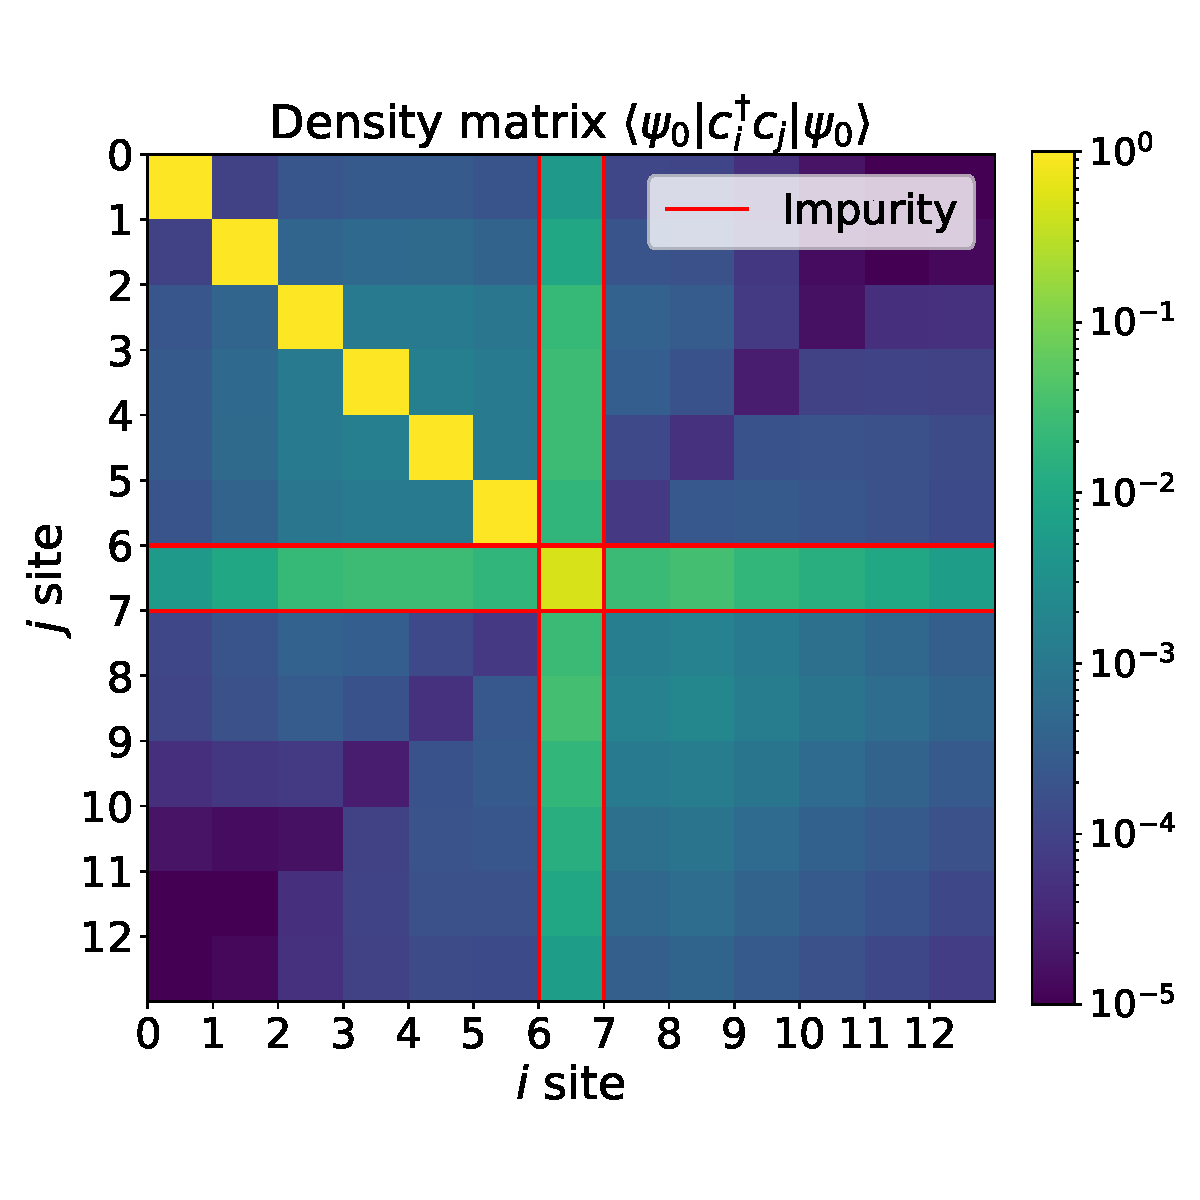
\includegraphics[width=1.05\textwidth, trim={0 1.7cm 0 1.6cm},clip]{imgs/dm.pdf}
\end{minipage}
\hspace{-0.1cm}
\begin{minipage}{0.38\textwidth}
\centering
	\begin{itemize}
		\item Benchmark with \textbf{no core states}.
		\item $\chi \sim 150$
		\item Bath sites $0-5$: valence sites.
		\item Bath sites $7-12$: conduction sites.
		\item \textbf{Impurity:} half-filled, correlated with all other bath sites.
	\end{itemize}
\end{minipage}


	\end{beamercolorbox}
	\end{block}
\end{column}

\begin{column}{.017\textwidth}
\end{column}	%Empty spacer column in the middle

\begin{column}{.23\textwidth}
	\begin{block}{\color{ta2orange!0}Lanczos Algorithm}
	\setbeamercolor{coloredboxstuff}{bg=ta2orange!0}
	\begin{beamercolorbox}[wd=\textwidth]{coloredboxstuff}
Projection of $\hat{H}$ in the Krylov subspace:
\begin{equation*}
\mathcal{K}_k(\hat{H}, v) = \text{span}(v, \hat{H}v, \ldots, \hat{H}^kv)
\end{equation*}

\begin{itemize}
	\item $v=T_a^\mathbf{q}|i\rangle$ the initial state
	\item $k\sim10^6$ the dimension of the subspace where diagonalisation is still manageable.
	\item Lanczos orthogonalizes the states iteratively.
\end{itemize}
\textbf{Problem}: applying $\hat{H}$ on a state increases the bond dimension $\chi$ significantly and thus the computational complexity...
	\end{beamercolorbox}
	\end{block}
\end{column}

\begin{column}{.03\textwidth}
\end{column} % Empty spacer column
\end{columns} % End of all the columns in the poster
\vspace{-0.75em}

%%%%%%%%%%%%%%%%%%%%%%%%%%%%%%%%%%%%%%%%%%%%%%%%%%%%%%%%%%%%%%%%%%
% Natural orbitals and ongoing
%%%%%%%%%%%%%%%%%%%%%%%%%%%%%%%%%%%%%%%%%%%%%%%%%%%%%%%


\begin{columns}[t]  % beginning of all the columns

\begin{column}{.03\textwidth}
\end{column} % Empty spacer column

\begin{column}{.58\textwidth} % The first column
\begin{block}{\color{cyan!40}Natural Orbitals\vphantom{Xy}}
\setbeamercolor{coloredboxstuff}{bg=cyan!5}
\begin{beamercolorbox}[wd=\textwidth]{coloredboxstuff}
salut

\end{beamercolorbox}
\end{block}
\end{column}

\begin{column}{.02\textwidth}
\end{column}	%Empty spacer column in the middle

\begin{column}{.36\textwidth} % The first column
\begin{block}{\color{ta2orange!30!tabutter!30} Conclusion and Outlook\vphantom{Xy}}
\setbeamercolor{coloredboxstuff}{bg=ta2orange!10!tabutter!10}
\begin{beamercolorbox}[wd=\textwidth]{coloredboxstuff}
coucou

\end{beamercolorbox}
\end{block}
\end{column}

\begin{column}{.03\textwidth}
\end{column} % Empty spacer column
\end{columns}
\vspace{-0.75em}

%%%%%%%%%%%%%%%%%%%%%%%%%%%%%%%%%%%%%%%%%%%%%%%%%%%%%%%%%%%%%%%%%%%%%%%%%%%%%%%%%%%%%%%%%%%%%%%%%%%%%%%%%%%%%%%%%%%%%%%%%

\begin{columns}[t]  % beginning of all the columns

\begin{column}{.03\textwidth}
\end{column} % Empty spacer column

\begin{column}{0.94\textwidth}
%
\begin{block}{\color{gray!10} \normalsize References}
{\footnotesize
\begin{thebibliography}{4}

\bibitem{Yavas2019}
H. Yavas, M. Sundermann, K. Chen, A. Amorese, A. Severing, H. Gretarsson, M. W. Haverkort, and L. H. Tjeng. \textit{Direct imaging of orbitals in quantum materials. Nature Physics}, 15(6) :559–562, 2019.

\bibitem{Baledent}
Right figure of the \textit{Motivation} box : experimental results of orbital imaging of copper oxide at $300$ K, by Victor Baledent and Jean-Pascal Rueff, with whom we are collaborating. The NRIXS spectra comes from paper \cite{Yavas2019} for NiO.

\bibitem{Tahir}
D. Tahir and S. Tougaard. \textit{Electronic and optical properties of Cu, CuO and Cu2O studied by electron spectroscopy. Journal of Physics: Condensed Matter, 24(17):175002, apr 2012.}

\bibitem{Marabelli}
F. Marabelli, G. B. Parravicini, and F. Salghetti-Drioli. \textit{Optical gap of CuO. Phys. Rev. B, 52:1433–1436, Jul 1995.}

\bibitem{ANR}
We gratefully acknowledge financial support from the ANR ClusterSpecs project.

\end{thebibliography}
 }
\end{block}
\end{column}

\begin{column}{.03\textwidth}
\end{column} % Empty spacer column
\end{columns}
%\vspace{-0.75em}

%%%%%%%%%%%%%%%%%%%%%%%%%%%%%%%%%%%%%%%%%%%%%%%%%%%%%%%%%%%%%%%%%%%%%%%%%%%%%%%%%%%%%%%%%%%%%%%%%%%%%%%%%%%%%%%%%%%%%%%%%


\end{frame} % End of the enclosing frame
\end{document}
